
%\frame{\titlepage}

\section{Wissen im Unternehmen}

\frame{
  \frametitle{Agenda}

  \tableofcontents
}

% Bedingt durch Globalisierung, Wettbewerb und Informationstechnik streben Unternehmen danach hochwertige Produkte und Dienstleistungen anzubieten
% Verschiebung d. Wirtschaft hin zum tertiären Sektor (Dienstleistungen) ~ 1950 32,5% \ldots 1975 51,0% \ldots 2011 73,8% (lt. Statistischem Bundesamt)
% Dafür sind die Mitarbeiter und deren Fähigkeiten die wichtigste Resource - Sie verfügen über ``Wissen''

\subsection{Einführung}
\frame{
  \frametitle{Einführung}
      Was ist Wissen?\\
      \vspace{0.2cm}
      Nur näherungsweise und im Kontext zu definieren\\
      \vspace{0.2cm}
      Ansätze:
      \begin{itemize}
         \item Nach Zugänglichkeit: Implizites und explizites Wissen
         \item Nach Personeller Bindung: Individuelles und kollektives Wissen
         \item Wissen vs. Information vs. Daten\\
           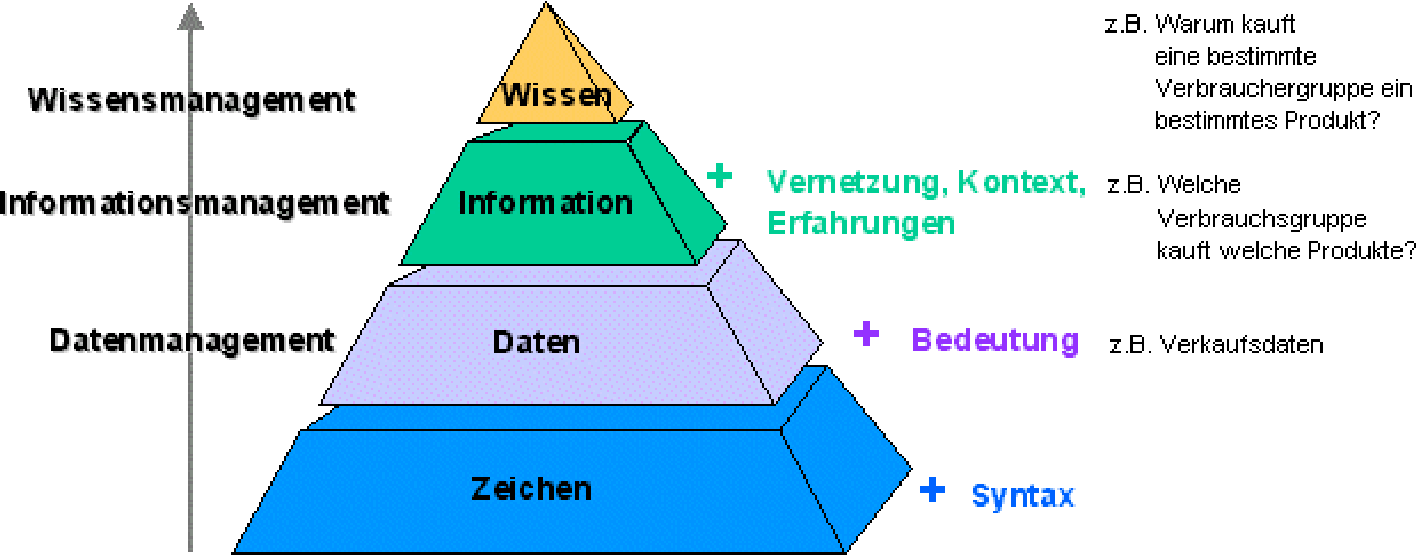
\includegraphics[width=0.5\textwidth]{images/wissenspyramide.png}
         \item ``Wissen ist in einen Kontext eingebettet und von ihm abhängig und kann daher nicht zeitlos objektiv sein.'' \cite{Schilcher:2006}
      \end{itemize}
  \vspace{0.1cm}  
  \begin{center}\small``Ich weiß, dass ich nichts weiß'' - Sokrates\end{center}
}
% ``Ich weiß, dass ich nicht[s] weiß'' ~ Sokrates
% Eine Definition des Begriffs ``Wissen'' ist kaum zu finden bzw. je nach Kontext und Autor verschieden
% Ansätze: 
% - Zugänglichkeit: Implizites und Explizites Wissen
% - Personelle Bindung: Individuelles und Kollektives Wissen
% - Wissen vs. Information (Sachverhalt unter best., def. Randbed. [Schmiede 1996a]) vs. Daten [vs. Zeichen]
%	Beispiel: Hilferuf am Badesee, Wechselkurs und Leitzinsänderungen
% - Wissen ist nicht ahistorisch, von sozialen & kulturellen Umständen abhängig (z.B. Maßeinheiten) ~ ``Wissen ist in einen Kontext eingebettet und von ihm abhängig und kann daher nicht zeitlos objektiv sein.'' [S. 18, Schilcher, C. - Implizite Dimensionen des Wissens und ihre Bedeutung für betriebliches Wissensmanagement, 2006]

\frame{
  \frametitle{Hauptformen des Wissens im Unternehmen}
  Hauptformen des Wissens im Unternehmen nach Franken \cite{Franken:2002}
  \begin{itemize}
    \item \textbf{Strukturiertes, formalisiertes Wissen} explizit und strukturiert, z.B. Datenbanken, ausgefüllte Formulare
    \item \textbf{Unstrukturiertes, formalisiertes Wissen} explizit und unstrukturiert, z.B. Bilder, Baupläne
    \item \textbf{Personelles Wissen} implizit, an Personen gebunden und durch Kommunikation vermittelbar
    \item \textbf{Kollektives Wissen} implizites, kulturelles Wissen
  \end{itemize}
  $\rightarrow$ Probleme im Umgang mit impliziten Wissensformen
}
% Franken: Hauptformen des Wissens in Unternehmen [Franken, Integriertes Knowledge Management]
% (S. 303)
% 1- Strukturiertes Wissen
% 2- Unstrukturiertes, formalisiertes Wissen
% 3- Personelles, individuelles Wissen
% 4- Kollektives Wissen
% Umgang mit 3 & 4 im Unternehmen nicht einfach -> Wissensmanagement erforderlich (wieder..)

\subsection{Motivation: Wissensmanagement}
\frame{
  \frametitle{Motivation: Wissensmanagement}
  Wozu Wissensmanagement?\\ \vspace{0.3cm}
  \begin{itemize}
    \item Kosten für externe Dienstleistungen verringern
    \item Verhindern doppelter Arbeit in verschiedenen Abteilungen
    \item Wissen im Unternehmen halten (auch bei Kündigung, Pensionierung, \ldots)
    \item Problemen des impliziten Wissens begegnen
  \end{itemize}
  
}
% Wozu Wissensmanagement? (S. 304)
% - Kompetenzen der Mitarbeiter kennen, nutzen (und ausbauen)..
%	.. da sonst:
%		- externe Dienstleistungen bezahlt werden, die In-House erledigt werden können
% - Austausch von Wissen innerhalb des Unternehmens..
%	.. da sonst:
%		- eine Abteilung etwas entwickelt, das eine andere Abteilung bereits fertiggestellt hat
% - IMHO Wichtigster Punkt:
% 	Sicherstellen, dass bei Kündigung, Pension etc. das Wissen im Unternehmen bleibt.
% -> Problemfall implizites Wissen
% 	Wie motiviere ich meine Mitarbeiter, Wissen weiterzugeben und von anderen anzunehmen?
% 		- Ideen sammeln? (Fragerunde?, Erfahrungen?, ..)
%		- Beispiel: Stellenabbau, Wissen über Verfahren weitergeben, aber an wen? und wie?
%		- ``Wissen ist Macht'' <-> Klima ausreichender Sicherheit und Offenheit schaffen, damit 'Hoheitswissen' geteilt wird

\frame{
  \frametitle{Kulturelle Unterschiede und der Wert des Impliziten}
  Nonaka und Takeuchi \cite{Nonaka:1997}
  \begin{itemize}
    \item In westlichen Unternehmen ist ``Wissen'' vor allem explizit.
    \item Japanische Unternehmen legen mehr Wert auf Implizites,\\
          z.B. Erfahrung, Intuition
  \end{itemize}
  \begin{center}
    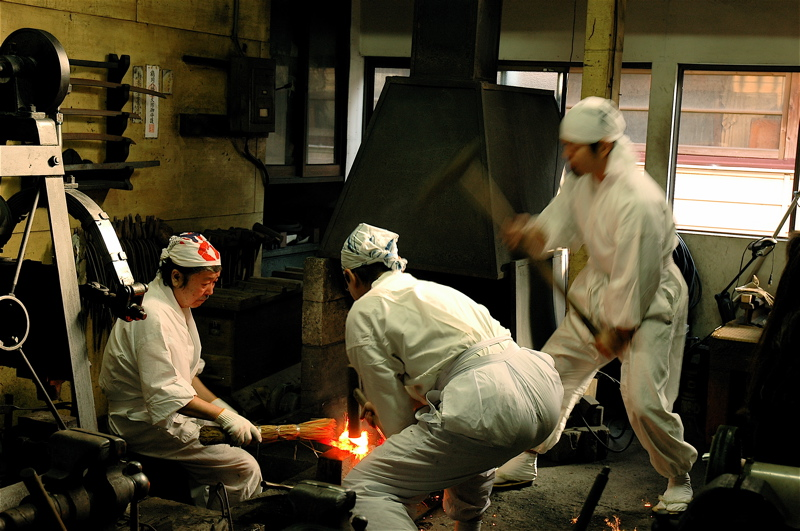
\includegraphics[width=0.6\textwidth]{images/kamakura-masamune-swordsmith-1.jpg} \cite{samurai}
  \end{center}
}
% Nonaka und Takeuchi: Kulturelle Unterschiede
% - Für westl. Unternehmen ist Wissen explizit. ``Explizites Wissen lässt isch in Worten und Zahlen ausdrücken und problemlos mit Hilfe von Daten, wissenschaflichen Formeln, festgelegten Verfahren oder universellen Prinzipien mitteilen'' [Nonake, Takeuchi, Die Organisation des Wissens]
% - Japan. Unternehmen ist der Stellenwert impliziten Wisses deutlich höher. ``Subjektive Einsichten, Ahnungen und Intuition fallen in diese Wissenskategorie. Darüber hinaus ist das implizite Wissen tief verankert in der Tätigkeit und deer Erfahrung des einzelnen sowie in seinen Idealen, Werten und Gefühlen'' [s.o.]

\subsection{Wissensmanagement}
\frame{
  \frametitle{Probst, Raub, Romhardt - Bausteine des Wissensmanagements \cite{Probst:2006}}
  \begin{columns}
    \column{0.5\textwidth}
      Gliederung in die Kernelemente
      \begin{itemize}
        \item Wissensidentifikation
        \item Wissenserwerb
        \item Wissensentwicklung
        \item Wissens(ver)teilung
        \item Wissensnutzung
        \item Wissensbewahrung
      \end{itemize}

    \column{0.5\textwidth}
      Ergänzt durch
      \begin{itemize}
        \item Wissensziele
        \item Wissensbewertung
      \end{itemize}

      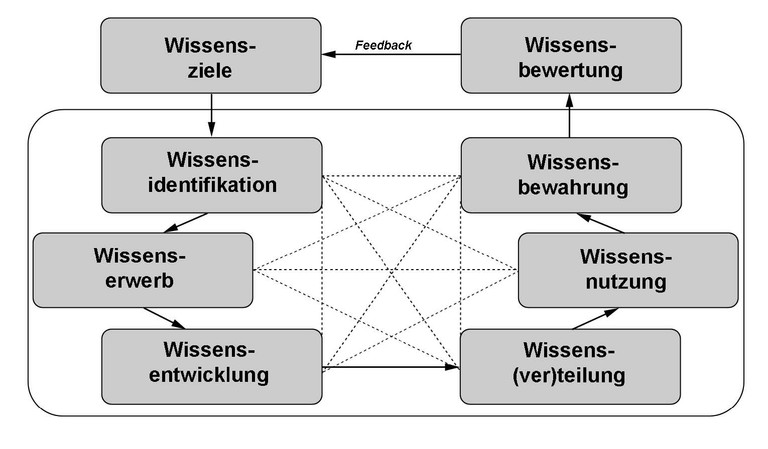
\includegraphics[width=0.8\textwidth]{images/probst.jpg}
  \end{columns}

  \begin{alertblock}{Kritik: Praxistauglichkeit}
    Hinweise zur Umsetzung fehlen. Wissensbewertung?
  \end{alertblock}
}
% G. Probst, S. Raub, K. Romhardt: ``Bausteine des Wissensmanagements'' [ebd. Wissen managen]
% Kernelemente: (S. 304)
% - Wissensidentifikation
% - Wissenserwerb
% - Wissensentwicklung
% - Wissens(ver)teilung
% - Wissensnutzung
% - Wissensbewahrung
% beschreiben die operativen Probleme des Umgangs mit Wissen im Unternehmen
% weiterhin
% - Wissensziele: Normativ (wissensbewusste Unternehmenskultur), Strategisch (zukünftigen Wissensbedarf definieren), Operativ (Umsetzung d. Wissensmanagement)
% - Wissensbewertung: Metriken, Bewertungskriterien finden, um Grad der Erfüllung o.g. Ziele zu messen \ldots nur wie?
% Kritik: Keine Hinweise auf praktische Umsetzung; Wissensbewertung (nahezu) unmöglich

\frame[allowframebreaks]{
  \frametitle{Wissensmanagement in der Praxis}
  Franken \cite{Franken:2007}
  \begin{itemize}
    \item Mitarbeiter steht im Mittelpunkt
    \item Voraussetzungen für freiwilliges Engagement schaffen
    \item Verhaltenskomponenten
      \begin{itemize}
        \item sollen
        \item dürfen
        \item können
        \item wollen
      \end{itemize}
  \end{itemize}
  Es bedarf der ``Befähigung, Fähigkeit und Bereitschaft zu lernen, Wissen anzunehmen sowie eigenes Wissen zu teilen'' \cite{Franken:2007}
  \framebreak

  Arbeitsbereiche des praktischen Wissensmanagements
  \begin{enumerate}
    \item \textbf{Wissensvision schaffen}
    \begin{itemize}
      \item Bild der Zukunft des Unternehmens vermitteln $\rightarrow$ ``sollen''
      \item Identifikation mit dieser Zukunft soll zu Engagement motivieren $\rightarrow$ ``wollen''
    \end{itemize}
    \item \textbf{Wissensgemeinschaft bilden}
    \begin{itemize}
      \item Förderung des individuellen Lernens z.B. in Workshops $\rightarrow$ ``können''
      \item Positive Einstellung gegenüber Neuerungen, Angstfreiheit, ``sinnvolle Fehlschläge'' tolerieren $\rightarrow$ ``dürfen''
    \end{itemize}
\framebreak
    \item \textbf{Interaktion unterstützen}
    \begin{itemize}
      \item Wissensaustausch fördern
      \item Offene Kommunikation und Vertrauen schaffen
    \end{itemize}
    \item \textbf{Erneuerungen fördern}
    \begin{itemize}
      \item Neue Teams zusammenstellen
      \item Nichtexperten einsetzen
      \item Ziel: Betrachtungsweisen in Frage stellen und neue gewinnen
    \end{itemize}
    \item \textbf{Middle-up-down-Management}
    \begin{itemize}
      \item Mittelweg zwischen hierarchischem und partizipativem Führungsstil
      \item ``Das implizite Wissen von oben (Visionen) und unten (Erfahrungen, Fertigkeiten und Intuition) verschmilzt und wird zum expliziten Wissen in Form von neuen Technologien, Produkten oder Programmen.'' \cite{Franken:2007}
    \end{itemize}
    \item \textbf{Hypertextorganisation}
    \begin{itemize}
        \item ..
    \end{itemize}
    \item \textbf{Wissensnetz mit der Außenwelt}
    \begin{itemize}
        \item ..
    \end{itemize}
  \end{enumerate}
}
% Franken (in Anlehnung an Nonaka und Takeuchi) - Wissensmanagement in der Praxis
% Voraussetzungen für das Verhalten der Mitarbeiter schaffen 
% ~ Verhaltenskomponenten:
%	``sollen'', ``dürfen'', ``können'' und ``wollen''
% - Mitarbeiter stehen im Mittelpunkt d. Wissensmanagements
% - Bedarf d. ``Befähigung, Fähigkeit und Bereitschaft zu lernen, Wissen anzunehmen sowie eigenes Wissen zu teilen'' [Franken, S. 307]
% - 

\subsection{Fazit \& Praxistipps}
\frame{
  \frametitle{Tools, Maßnahmen}
  \begin{itemize}
    \item ``Wissen ist Macht'' überwinden
    \item Dokumentation
    \item Wikis
    \item stackoverflow
    \item Kommunikation
    \item Vorträge von internen und externen Experten
    \item Einbeziehung fachfremder Personen
    \item Aufgeschlossenheit gegenüber Kreativität und Neuerungen
  \end{itemize}
}

\frame{
  \frametitle{Fazit}
%    \begin{itemize}
%      \item Implizite Wissen verteilen und (wenn möglich) formalisieren
%      \item Aufgeschlossenheit gegenüber Kreativität und Neuerungen 
%      \item ``Tools'' z.B. Wikis, Blogs, stackoverflow, \ldots
%      \item Events als Kommunikationsgelegenheit
%      \item Vorträge von Mitarbeitern für Mitarbeiter
%      \item \ldots
%    \end{itemize}
}
%\subsection{Einführung}
%\frame{
%  \frametitle{Einführung}
%  \begin{itemize}
%    \item Trend zur Wissensarbeit
%    \item ``Immaterielle'' Wertschöpfung
%    \item Metapher: Fabrik $\rightarrow$ Küche
%  \end{itemize}
%}

%\subsection{Definition: Wissen}
%\begin{frame}[allowframebreaks]
%\frametitle{Definition: Wissen}
%\begin{description}
% \item[Zeichen] Symbole, kontextfrei
% \item[Daten] Verkettung von Zeichen, frei von einem Verwendungszweck
% \item[Informationen] Daten im Kontext eines Problemzusammenhangs
% \item[Wissen] Eine Menge von Informationen, Modellierte Wirklichkeit
%\end{description}
%\textbf{Beispiel}: Wechselkurse %``1'' ``,'' ``4'' ``9'' $\rightarrow$ ``1,49'' $\rightarrow$ ``1,49 EUR/USD'' $\rightarrow$ Verhalten von Kursen angesichts von Leitzins, Markt, \ldots
%\framebreak
%\begin{description}
% \item[Explizit] Regeln, Texte
% \item[Implizit] Intuitives Handeln, Wiedererkennen bekannter Situationen
%\end{description}
%\end{frame}

%\subsection{Wissensgenerierung}
%\begin{frame}{Wissensgenerierung}
%Intern
%\begin{itemize}
% \item Forschung und Entwicklung
% \item Anreize zum Wissenstransfer
% \item Technische Infrastruktur
%\end{itemize}
%Extern
%\begin{itemize}
% \item Forschungskooperationen
% \item Lead-User
% \item Lieferanten-Kunden-Netzwerk
%\end{itemize}
%\end{frame}



